\documentclass[conference]{IEEEtran}
\IEEEoverridecommandlockouts

\usepackage{cite}
\usepackage{amsmath,amssymb,amsfonts}
\usepackage{graphicx}
\usepackage{textcomp}
\usepackage{xcolor}

\usepackage{subcaption}

\usepackage{tikz}
\usepackage{pgfplots}

\usepackage{cleveref}
\usepackage{csquotes}
\usepackage{booktabs}

\usepackage{flushend}


\definecolor{tol1}{HTML}{33bbee}
\definecolor{tol2}{HTML}{009988}
\definecolor{tol3}{HTML}{ee7733}
\definecolor{tol4}{HTML}{cc3311}

\usepackage{acro}
\DeclareAcronym{cots}{
  short = COTS,
  long = off-the-shelf,
}

\DeclareAcronym{tiff}{
  short = TIFF,
  long = tag image file format,
}

\DeclareAcronym{mse}{
  short = MSE,
  long = mean squared error,
}

\DeclareAcronym{awgn}{
  short = AWGN,
  long = additive white Gaussian noise,
}

\DeclareAcronym{leo}{
  short = LEO,
  long = low Earth orbit,
}

\DeclareAcronym{ldpc}{
  short = LDPC,
  long = low-density parity-check,
}

\DeclareAcronym{jscc}{
  short = JSCC,
  long = joint source and channel coding,
}

\DeclareAcronym{djscc}{
  short = DJSCC,
  long = deep joint source and channel coding,
}

\DeclareAcronym{snr}{
  short = SNR,
  long = signal-to-noise ratio,
}

\DeclareAcronym{cnn}{
  short = CNN,
  long = convolutional neural network,
}

\DeclareAcronym{psnr}{
  short = PSNR,
  long = peak signal-to-noise ratio,
}

\DeclareAcronym{prelu}{
  short = PReLU,
  long = parameterized rectified linear unit,
}

\DeclareAcronym{jscc-sat}{
  short = \textsc{JSCC-Sat},
  long = {joint source-and-channel coding for small satellite applications}
}

\DeclareAcronym{los}{
  short = {LOS},
  long = {line of sight}
}

\DeclareAcronym{esa}{
  short=ESA,
  long=European Space Agency
}

\usepackage{xspace}
\newcommand\cubesat{CubeSat\xspace}
\newcommand\cubesats{\cubesat{}s\xspace}

\newcommand\jpegtwok{JPEG\,2000\xspace}

\newcommand\sentinelii{Sentinel-2\xspace}

\begin{document}

\title{Adaptable Joint Source-and-Channel Coding for Small Satellite Applications}

\author{\emph{Anonymous authors}}
% \author{\IEEEauthorblockN{Olga Kondrateva}
% \IEEEauthorblockA{\textit{Humboldt-Universit\"at zu Berlin}\\
% Berlin, Germany \\
% kondrate@informatik.hu-berlin.de}
% \and
% \IEEEauthorblockN{Stefan Dietzel}
% \IEEEauthorblockA{\textit{Merantix Momentum GmbH}\\
% Berlin, Germany \\
% stefan@merantix-momentum.com}
% \and
% \IEEEauthorblockN{Bj\"orn Scheuermann}
% \IEEEauthorblockA{\textit{Technical University of Darmstadt}\\
% Darmstadt, Germany \\
% scheuermann@kom.tu-darmstadt.de}
% }

\maketitle

\begin{abstract}
Earth observation using small satellites serves a wide range of relevant applications.
However, significant advances in sensor technology (e.g., higher resolution, multiple spectrums beyond visible light) in combination with challenging channel characteristics lead to a communication bottleneck 
when transmitting the collected data to Earth.
Recently, joint source coding, channel coding, and modulation using a neuronal-network-based approach has been proposed to combine image compression and communication. %dynamically adapt to the varying communication channel and to take data properties into account.
Though this approach achieves promising results when applied to standard terrestrial channel models, 
it remains an open question whether it is suitable for the more complicated and quickly varying satellite communication channel. 
In this paper, we consider a detailed satellite channel model accounting for different shadowing conditions and train an encoder-decoder architecture using realistic \sentinelii satellite imagery.
In addition, to reduce the overhead associated with using multiple neural networks for various channel states, 
we leverage attention modules and train a single adaptable neural network that covers a wide range of different channel conditions.
Our evaluation results show that the proposed approach achieves on-par performance when compared to less space efficient schemes using separate neuronal networks for differing channel conditions.   
% it typically involves training multiple neural networks to account for different channel conditions  
% In this paper, we propose a novel joint coding scheme that combines image compression, channel coding, and modulation using a neuronal-network-based approach.
% By combining a detailed channel model for small satellite applications with attention modules, we can use a single adaptable neuronal network to cover a wide range of different channel conditions.
% We evaluate our approach using realistic \sentinelii satellite imagery and show that it achieves on par performance when compared to less space efficient schemes using separate neuronal networks for differing channel conditions.
\end{abstract}

\begin{IEEEkeywords}
  cross-layer optimization; AI-enabled networking; small satellite applications
  \end{IEEEkeywords}

\acresetall
\section{Introduction}

Earth observation using sensor data acquired by satellites has gained more and more attention over the last years.
Common use cases include environment monitoring \cite{rs14030589}, disaster management \cite{barmpoutis2020}, and many more \cite{radix,MarCO}.
The increasing momentum can be explained by two major factors.
First, technological advances have allowed to build smaller satellite classes, which use more off-the-shelf components and can be deployed more easily.
A prime example are CubeSats, which operate in \ac{leo} and consist of $10 \times 10 \times 10$\,cm units \cite{cubesat2020}.
Second, sensor technology has improved greatly.
Besides higher resolution, modern sensors support a wider spectrum range, exceeding that of visible light.
Hyper-spectral images include infrared and other bands, which can be used monitor vegetation, clouds, and other phenomena not represented in the visible light spectrum.

These advances in satellite and sensor technology, however, are not met by an equal improvement in communication capacity.
CubeSats and other small satellites have a constrained energy budget, and -- unlike their larger counterparts -- they are not geo-stationary.
That is, they orbit the Earth several times per day with high speed, limiting communication with ground stations to several short communication windows.
Their high velocity and interferences due to harsh weather and potential non line-of-sight conditions further lead to high packet loss rates and complicate communication \cite{nogales2018}.

Therefore, efficient and robust coding schemes are a necessity to support demanding Earth observation applications.
Typically, source coding, channel coding, and modulation schemes are combined to translate image sensor data into physical layer channel symbols.
Source coding serves to compress sensor images, often using lossy compression schemes, such as \jpegtwok \cite{sentinel-2-user-handbook}.
Channel coding (e.g., \ac{ldpc}) is then used to enable error correction, counteracting packet loss due to the harsh channel conditions.
More recently, approaches that consider these coding mechanisms jointly have emerged, promising better than performance than using individual coding schemes \cite{6408177}.
Joint coding leverages the data-centric nature of the considered use case: the characteristics of the hyper-spectral image sensor data is well known, and therefore, the image data can be translated directly into physical layer symbols rather than using separate source codes, channel codes, and modulation.
And although Shannon's theory \cite{cover1991elements} states that separate optimization should yield optimal results, this is not true in practice due to hypothetical assumptions, such as infinite code block lengths.

The use of neuronal networks has provided a feasible way to implement such a joint coding approach, improving over earlier work, which was too complex to be useful in practice \cite{9838671}.
Neuronal-network-based joint coding approaches have been proposed for both terrestrial communication \cite{Bourtsoulatze2019} and satellite applications \cite{satjscc}.
So far, a major limitation has been that the joint encoder and decoder has been trained based on fixed assumptions about channel characteristics, such as the \ac{snr} using a simple \ac{awgn} channel model.
To accommodate changing channel conditions, separate neuronal networks need to be trained independently and switched between by both the satellite and the ground station.
Obviously, this approach restricts the total number of channel parameter combinations that can reasonably be covered.
Considering more complex channel models including multi-path propagation, shadowing, and fading would easily lead to a combinatorial explosion of parameters, and consequently a prohibitive amount of separate neuronal networks.

In this paper, we propose a novel joint coding approach for satellite applications that allows to use a single neuronal network for a wide range of channel conditions typical for small satellite applications.
We use a neuronal network model architecture that is enriched by so-called attention modules to reduce the combinatorial complexity.
Using this architecture, we can train a single neuronal network based on a number of different channel conditions.
During operation, the attention modules allow to essentially parametrize the network for different actual channel conditions.
This parametrization allows us to consider a wide range of realistic channel conditions for small satellite applications.
To model the channel, we use Fontán et al.'s channel model \cite{fontan2001}, which is applicable to non-geostationary small satellites and models a number of channel characteristics, such as multi-path propagation and shadowing.
More specifically, we consider three scenarios -- \ac{los}, shadowing, and deep shadowing -- to capture different extents of multi-path propagation and shadowing effects.
In addition, we also consider different levels of \ac{snr} to model satellite elevation angles and other parameters.
During training of the encoder-decoder neuronal network, these parameters are used as input, in addition to a large number of example satellite images.
Whereas a traditional encoder-decoder network would then -- simply speaking -- learn a coding scheme for the \enquote{average} of all parameters, the attention modules allow to embed schemes for all parameters within a single network that can be dynamically parameterized with the actual channel conditions during use.
Therefore, a single network suffices when using attention modules, and separate networks with a simpler architecture are required in order to precisely represent different channel conditions.
Although the resulting network with attention modules is larger than one trained for a specific set of channel conditions, it is considerably smaller than considering a set of separate networks, one for each channel condition.

Our evaluation using a set of hyper-spectral images from the \sentinelii mission shows that our approach performs as good as separate, individual networks for different channel conditions while requiring significantly lower storage overhead.

Thus, our main contributions can be summarized as follows:
%
\begin{enumerate}
  \item We combine \ac{jscc} approaches with a realistic channel model for small satellite applications.
  \item We apply an attention-module-augmented neuronal network architecture to be able to use a single network for a wide range of realistic channel characteristics.
  \item We evaluate our approach using a set of realistic \sentinelii Earth observation data.
\end{enumerate}

The remainder of this paper is organized as follows.
In \Cref{sec:related_work}, we review existing work on \ac{jscc}, source coding, channel models, and attention modules.
Next, we provide an overview of our system model in \Cref{sec:system_model} before explaining our mechanism in detail in \Cref{sec:our_approach}.
\Cref{sec:evaluation} details our evaluation results using \sentinelii mission data.
We conclude the paper in \Cref{sec:conclusion}.

\section{Related Work}
\label{sec:related_work}

\begin{itemize}
  \item LCN23
  \item Channel models for satellites
  \item Attention modules
\end{itemize}



\section{Earth Observation Missions}
\label{sec:system_model}

\begin{figure*}
  \begin{subfigure}{.32\linewidth}
    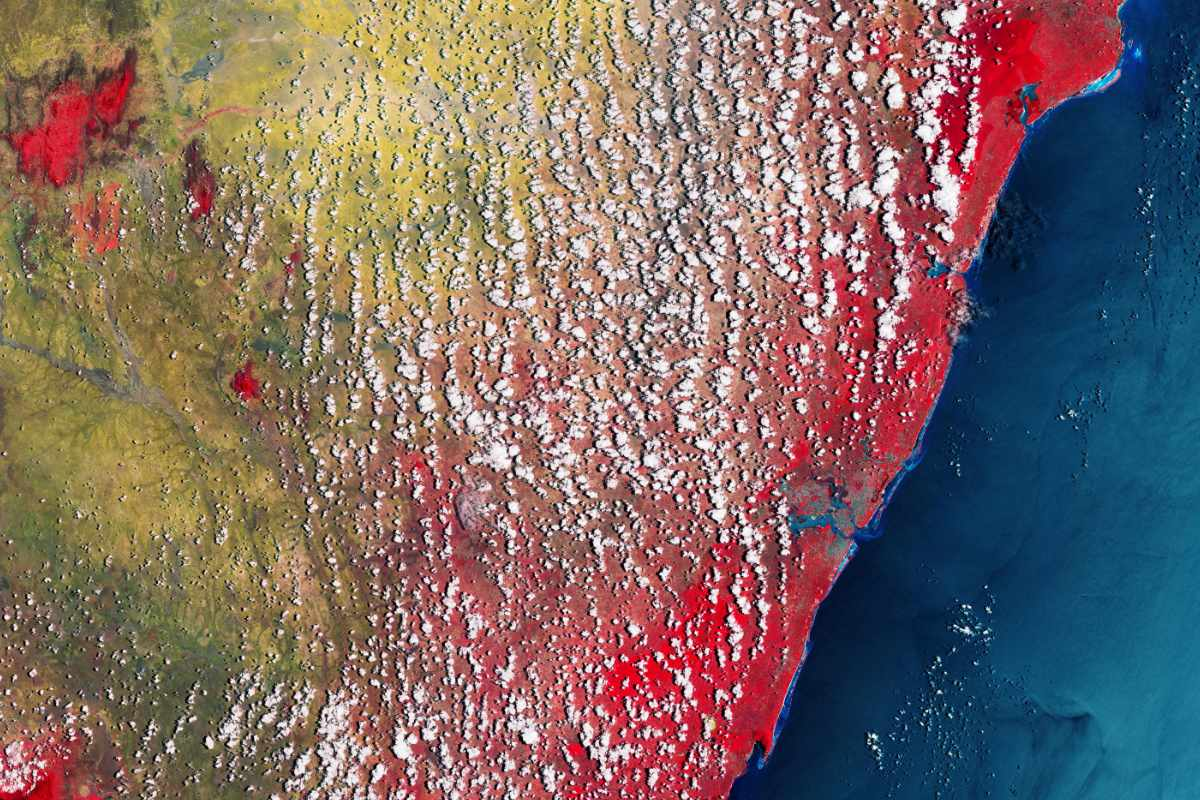
\includegraphics[width=\linewidth]{figures/Earth_from_Space_Southeast_Kenya}
    \caption{Southeast Kenya}
    \label{fig:sentinel_kenya}
  \end{subfigure}
  \hfill
  \begin{subfigure}{.32\linewidth}
    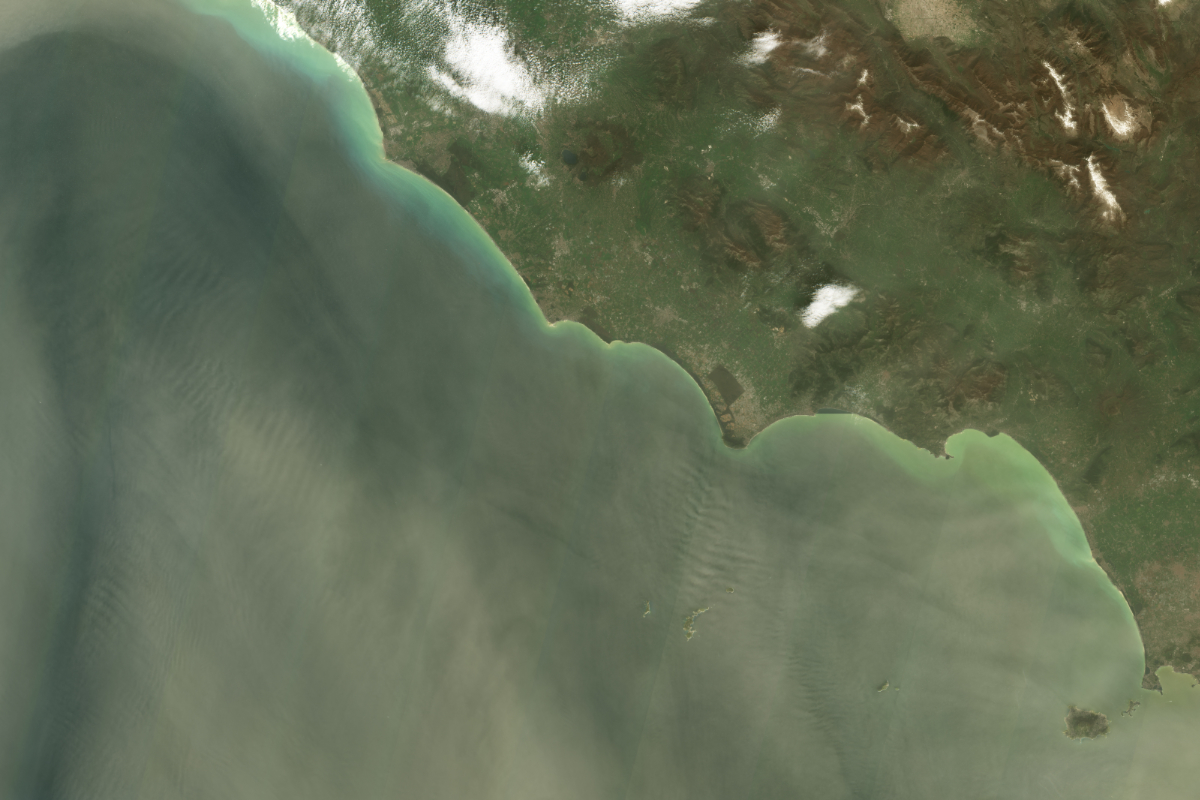
\includegraphics[width=\linewidth]{figures/Saharan_dust_plume}
    \caption{Sahara dust}
    \label{fig:sentinel_sahara}
  \end{subfigure}
  \hfill
  \begin{subfigure}{.32\linewidth}
    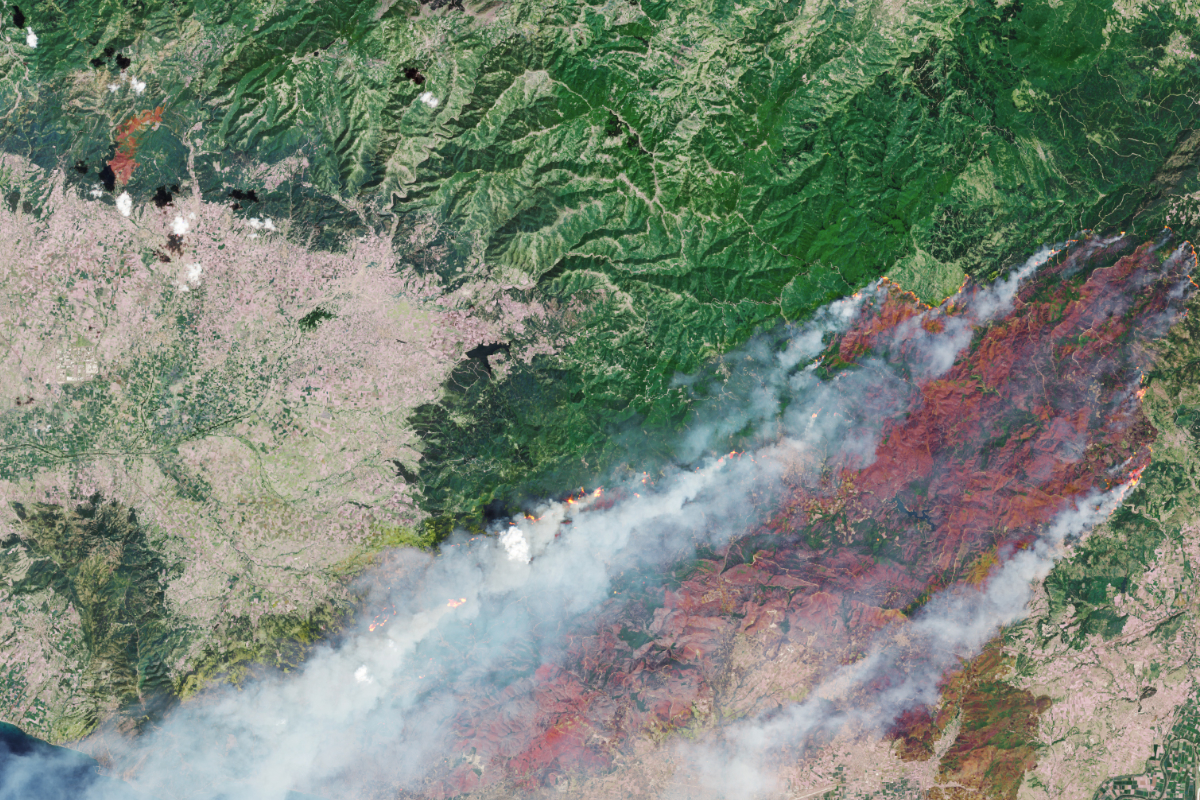
\includegraphics[width=\linewidth]{figures/Wildfires_continue_to_rage_in_Greece}
    \caption{Wildfires in Greece}
    \label{fig:sentinel_greece}
  \end{subfigure}

  \caption{Example images from the \sentinelii mission. (Credit: processed by ESA, CC BY-SA 3.0 IGO)}
  \label{fig:sentinelii}
\end{figure*}

\begin{table}
  \caption{\sentinelii Spectrum Bands}
  \label{tab:sentinel_bands}

  \centering
  \begin{tabular}{llcc}
    \toprule
    Band & Measurement & Central wavelength & Resolution \\
    \midrule
    1 & Coastal aerosol & 443 nm & 60 m \\
    2 & Blue & 490 nm & 10 m \\
    3 & Green & 560 nm & 10 m \\
    4 & Red & 665 nm & 10 m \\
    5 & Vegetation red edge & 705 nm & 20 m \\
    6 & Vegetation red edge & 740 nm & 20 m \\
    7 & Vegetation red edge & 783 nm & 20 m \\
    8 & Near infrared & 842 nm & 10 m \\
    8A & Narrow near infrared & 865 nm & 20 m \\
    9 & Water vapour & 940 nm & 60 m \\
    10 & Short wave infrared: cirrus & 1375 nm & 60 m \\
    11 & Short wave infrared & 1610 nm & 20 m \\
    12 & Short wave infrared & 2190 nm & 20 m \\
    \bottomrule
  \end{tabular}
  
\end{table}

With recent advances in space and image sensing technologies, Earth observation using small satellites has gained more and more attention over the past years.
As an example use case for the methods we propose in this paper, we briefly introduce ESA's \sentinelii mission.
We also use a subset of the mission's dataset for our evaluation.
Moreover, we give an overview of how neuronal networks are used onboard satellites for image processing.

\sentinelii \cite{sentinel2} is a set of missions operated by the \ac{esa} as part of the Copernicus program using \ac{leo} satellites.
The first satellites were launched in 2015, with more launches following in 2017 and 2024.
The missions comprise two satellites, which orbit the Earth such that each spot on the surface is revisited approximately every five days.
With their sensors, they cover a strip of land that is 290 km wide with each pass.
In addition to visible light sensors, the satellites are equipped with sensors that cover additional frequencies, such as infrared \cite{sentinel-2-user-handbook}, which allow to capture land use and vegetation (cf. \Cref{tab:sentinel_bands}).
Moreover, the sensors feature relatively high optical resolutions between 10 and 60 meters.

% https://www.esa.int/ESA_Multimedia/Images/2024/03/Earth_from_Space_Southeast_Kenya
% https://www.esa.int/ESA_Multimedia/Images/2024/04/Saharan_dust_plume
% https://www.esa.int/ESA_Multimedia/Images/2023/08/Wildfires_continue_to_rage_in_Greece

\Cref{fig:sentinelii} shows three example use cases for Earth observation images taken from \ac{esa}'s homepage.
The first (\Cref{fig:sentinel_kenya}) is a false-color image of southeast Kenya, which was generated by overlaying \sentinelii's near-infrared channel onto the visual spectrum.
The bright red colors indicate higher plant density and health, as alive plants reflect near-infrared light.
Thereby, the dense vegetation in the coastal regions can easily be distinguished from the hinterland regions.
\Cref{fig:sentinel_sahara} shows a dust storm originating from the Sahara desert.
\sentinelii provides valuable insights for air pollution monitoring, and due to the short revisit time, storms can be monitored as they develop.
Finally, \Cref{fig:sentinel_greece} shows wildfires in Greece in 2023.
For the visualization, the shortwave infrared spectrum was merged with the visible light spectrum, showing the fire front.
Dark brown areas show the burned area.
Thereby, these images provided valuable insights for civil protection authorities.
By using more efficient and more robust image compression and transmission, sensor data in small satellite missions can be transmitted and used faster, allowing even more rapid responses.

In this paper, we propose a neuronal-network-based \ac{jscc} approach to improve communication.
As small satellites are severely power-constrained, necessary hardware resources need to be taken into account when considering the feasibility of our solution.
Recently, a number of processing platforms have been successfully evaluated for use in space and small satellite applications.
Two examples are the Intel Movidius Myriad 2 and STM32 Microcontrollers, which have been used to identify stars and only use approximately 1 Watt power \cite{8556744}.
During the $\Phi$-Sat mission, deployment of machine learning models has been evaluated using an Intel Movidius Myriad processor, as well.
Similarly, Nvidia's TX2 SoC, which is compatible with the CubeSat standard's power constraints, has been used to detect cargo ships \cite{8556744}.
Finally, even relatively large standard machine learning models, such as VGG19 \cite{DBLP:journals/corr/SimonyanZ14a} and ResNet50 \cite{7780459}, have been evaluated on the International Space Station (ISS), operating on the Qualcomm Snapdragon 855 and Intel Movidius Myriad X processors \cite{9884906}.


\section{Our Approach}
\label{sec:our_approach}

The goal of our approach is to transmit sensor data $x \in \mathbb{R}$ acquired by small satellites in \ac{leo} to a ground station over a bandwidth-constrained channel.
The sensor data comprises optical images from multiple spectrums as defined in \Cref{sec:system_model}.
Assuming lossy compression and transmission, the ground station reconstructs an approximation $\hat{x}$ of the original data $x$ with the goal that $\hat{x}$ is as close to $x$ as possible.
Next, we given an overview of the protocol architecture before we explain the neural network architecture using attention modules and the channel model in more detail.

\subsection{Architecture overview}

\begin{figure}
  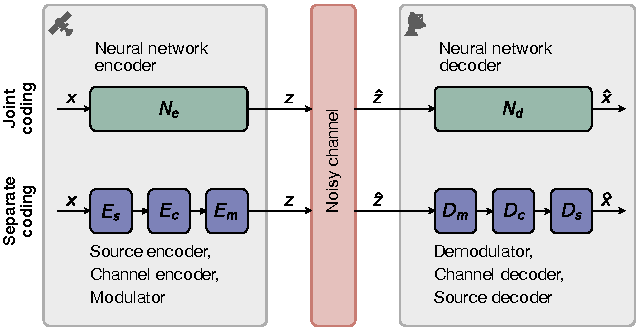
\includegraphics[width=\linewidth]{figures/coding-decoding}

  \caption{Overview of our communication architecture and comparison with traditional separate-encoder designs.}
  \label{fig:overview}
\end{figure}

To introduce our protocol's main components, we first explain the basic \ac{jscc} communication architecture and contrast it to the traditional case that uses separate encoders and decoders.
\Cref{fig:overview} shows an overview of the architecture in contrast to traditional approaches.
With separate coding (shown in the bottom half), the sensor data $x \in \mathbb{R}^n$ is first encoded using a source encoder, such as \jpegtwok.
Afterwards, a channel encoder (e.g., \ac{ldpc}) adds redundancy to the compressed signal in order to protect it against packet loss due to interference.
The modulator component then translates the channel encoder's output to physical layer samples $z \in \mathbb{C}^k$, which can be transmitted over a noisy channel.
The ground station receives the distorted signal $\hat{z}$ and uses corresponding components in inverse order to decode an approximation of $x$.
The demodulator $D_m$ translates the samples back to bits, which serve as input to the channel decoder $D_c$.
The channel decoder reconstructs the compressed image data, correcting transmission errors as far as possible.
The source decoder $D_s$ finally approximately reconstructs the original optical sensor data as $\hat{x}$.

In our \ac{jscc} approach (upper half of \Cref{fig:overview}), in contrast, parts of a single neuronal network are used as encoder $N_e$ and decoder $N_d$ by the satellite and ground station, respectively.
These components jointly perform the source coding, channel coding, modulation, and their corresponding inverse operations.

We use an encoder-decoder neuronal network architecture based on \cite{satjscc} to implement $N_e$ and $N_d$:
During training, the encoder ($N_e$) and decoder ($N_d$) parts of the network are linked together using a realistic channel model for noisy satellite links.
To better reflect realistic channel conditions, we replace the \ac{awgn} channel used in \cite{satjscc} with a more realistic channel model for \ac{leo} satellites.
The encoder-decoder model is then trained using an image dataset derived from the body of \sentinelii mission data.
The images within the dataset are used as model input and the reconstructed image's quality is used as reward metric.
Normally, a separate model would need to be trained for each characteristic set of channel conditions \cite{satjscc}.
In order to use a single network for a wide array of channel conditions, we augment the model with so-called attention modules \cite{wireless-attention-modules} as part of both the encoder and decoder during training.
These essentially allow to parameterize the network during later operation to cater to changing channel conditions.
The trained network is then separated into the encoder component $N_e$, which is used by the satellite and the decoder component $N_d$, which is used by the ground station.

\subsection{Encoder-decoder architecture with attention modules}

\begin{figure}
  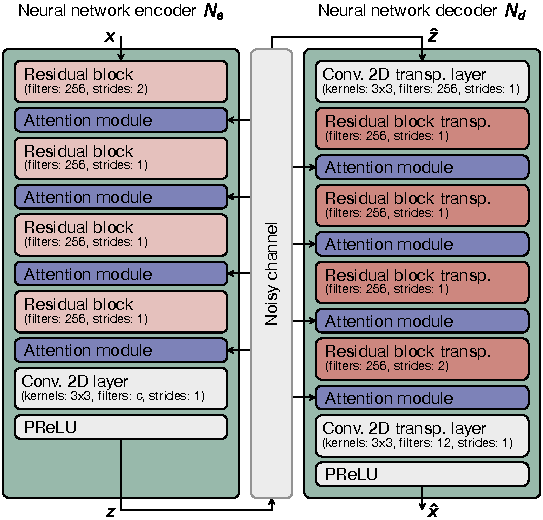
\includegraphics[width=\linewidth]{figures/network-architecture}

  \caption{Network architecture overview.}
  \label{fig:architecture-overview}
\end{figure}

The encoder-decoder network architecture is shown in \Cref{fig:architecture-overview}.
As basis, we use the network structure proposed in \cite{satjscc}, which adapts ResNet \cite{resnet} to the \ac{jscc} use case.
To make the architecture more flexible, we add attention modules, as well as a more realistic channel model.
The block on the left serves as neural network encoder, jointly performing source coding, channel coding, and modulation.
Compression is achieved by translating the input $x \in \mathbb{R}^n$ to channel symbols $z \in \mathbb{C}^k$, where $k < n$.
By adjusting $k$, the system's compression ratio $k/n$ can be defined.

\begin{figure*}
  \begin{subfigure}{.3\linewidth}
    \centering
    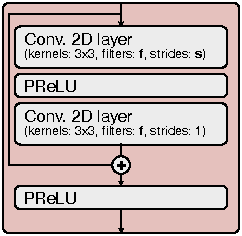
\includegraphics[height=10em]{figures/residual-block}
    \caption{Residual block $(f, s)$}
    \label{fig:residual}
  \end{subfigure}
  \hfill
  \begin{subfigure}{.3\linewidth}
    \centering
    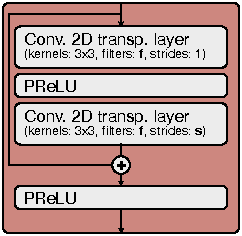
\includegraphics[height=10em]{figures/residual-block-transpose}
    \caption{Residual block transpose $(f, s)$}
    \label{fig:residual-transpose}
  \end{subfigure}
  \hfill
  \begin{subfigure}{.3\linewidth}
    \centering
    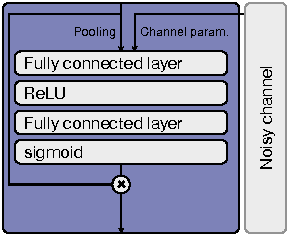
\includegraphics[height=10em]{figures/attention-module}
    \caption{Attention module}
    \label{fig:attention}
  \end{subfigure}

  \caption{Specific block architectures used within the encoder-decoder network.}
  \label{fig:blocks}
\end{figure*}

For the encoder, we use four residual blocks with 256 filters and a kernel size of $3 \times 3$.
The structure of the residual blocks is shown in \Cref{fig:residual}.
Each residual block is followed by an attention module as proposed in \cite{wireless-attention-modules}.
\Cref{fig:attention} shows the structure of the attention modules.
These modules allow to alter the feature weights of their preceding residual blocks in order to accommodate different channel conditions.


%%%% TODO REWRITE FROM HERE %%%%


AF module takes the SNR and the output of the FL module as the input and produces a sequence of scaling parameters. The product of the outputs of the FL module and the AF module can be seen as a filtered version of the FL module output.

The channel relationship are captured and different scaling parameters are generated for different channel features to increase or suppress their connection strength to the next layer. The aforementioned mechanism is channel-wise soft attention1 .

1) context extraction; 2) factor prediction; and 3) feature recalibration

1) global average pooling on output to extract global information, concatenate with channel params
2) use simple structure with fcl to predict feature importance based on channel params
3) calibrate feature importance based on fcl output

The last layer is a convolutional layer consisting of $c$ filters, where $c$ is determined by the compression ratio $k/n$.
We use a \ac{prelu} as activation function, which generalizes the traditional ReLU by introducing a learnable parameter, which improves predictions.
The output of the encoder is combined into a vector $\tilde{z}$ of $k$ complex-valued numbers representing the channel symbols.

The next layer is a non-trainable channel layer that gives a realistic representation of ... channel model ... see \Cref{sub:channel_model}.

The block on the right serves as neural network decoder, which translates the -- potentially corrupted channel symbols $\hat{z}$ back to an approximation $\hat{x}$ of the original data.

Similar to encoder, the decoder consists of a convolutional transpose layer, four residual transpose blocks (see \Cref{fig:residual-transpose}), another convolutional transpose layer, and a \ac{prelu} activation function.

During evaluation, use the \ac{psnr} as a metric to determine the quality of the reconstructed image as follows:
%
\begin{equation}
  \mathrm{PSNR} = 10 \log_{10}\frac{\mathrm{MAX}^2}{\mathrm{MSE}},
\end{equation}
%
where $\mathrm{MAX}$ is the maximum possible pixel value.

Intuitively, \ac{psnr} expresses the ratio between the maximum possible signal value and the distorting noise that reduces its quality.
The metric is often used to measure the reconstruction quality of lossy compression codecs, as it approximates human perception of the reconstruction quality.


\subsection{Channel model for \ac{leo} satellites}
\label{sub:channel_model}


\subsection{Attention Modules}

anderes paper zusammen fassen

\section{Evaluation}
\label{sec:evaluation}

\section{Conclusion}
\label{sec:conclusion}

\bibliographystyle{IEEEtran}
\bibliography{references}

\end{document}
